\documentclass[11pt,a4paper]{article}

% These are extra packages that you might need for writing the equations:
\usepackage{amsmath}
\usepackage{amsfonts}
\usepackage{amssymb}
\usepackage{booktabs}
\usepackage{hyperref}
\usepackage{listings}
\usepackage{xcolor}
\lstset {language=C++,
		 basicstyle=\ttfamily,
         keywordstyle=\color{blue}\ttfamily,
         stringstyle=\color{red}\ttfamily,
         commentstyle=\color{purple}\ttfamily,
         morecomment=[l][\color{magenta}]{\#},
       	 basicstyle=\tiny}

% You need the following package in order to include figures in your report:
\usepackage{graphicx}

% With this package you can set the size of the margins manually:
\usepackage[left=2cm,right=2cm,top=2cm,bottom=2cm]{geometry}


\begin{document}

% Enter the exercise number, your name and date here:
\noindent\parbox{\linewidth}{
 \parbox{.25\linewidth}{ \large ICP, Exercise 01 }\hfill
 \parbox{.5\linewidth}{\begin{center} \large Beat Hubmann \end{center}}\hfill
 \parbox{.2\linewidth}{\begin{flushright} \large Sep 30, 2018 \end{flushright}}
}
\noindent\rule{\linewidth}{2pt}


\section{Introduction}

Several small experiments on a basic congruential random number generator were conducted.

\section{Algorithm Description}
The congruential random number generator employed generates pseudo-random numbers $x_i$ based on the linear recurrence relation $x_{i+1} = (c \cdot x_i)\; \text{mod} \; p \: \text{where} \: c, p \in \mathbb{R} $~.

\section{Results}

\subsection{Task 1}

\subsubsection{Subtask 1.1}
200 random numbers were generated using $c = 3, \: p = 31$ and plotted for the square test. As shown in figure~\ref{fig:1a}, three lines were observed after normalizing the generated numbers with $x_i \gets \frac{x_i}{p}$.


\begin{figure}[ht]
\begin{center}
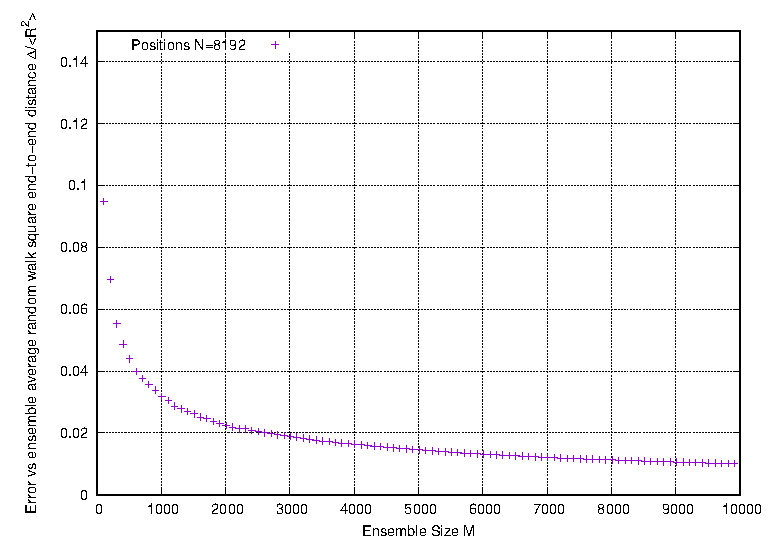
\includegraphics[scale=0.9]{figure1a.eps} 
\end{center}
\caption{Square test for congruential random number generator with $c = 3, \: p = 31$.}
\label{fig:1a}
\end{figure}


\subsubsection{Subtask 1.2}
As in the previous task, 200 random numbers were generated using $c = 3, \: p = 31$ and plotted for the cube test. As shown in figure~\ref{fig:1b}, regular patterns can be observed after normalizing the generated numbers with $x_i \gets \frac{x_i}{p}$, but identifying planes is somewhat difficult owing to the spacing caused by the short period.

\begin{figure}[ht]
\begin{center}
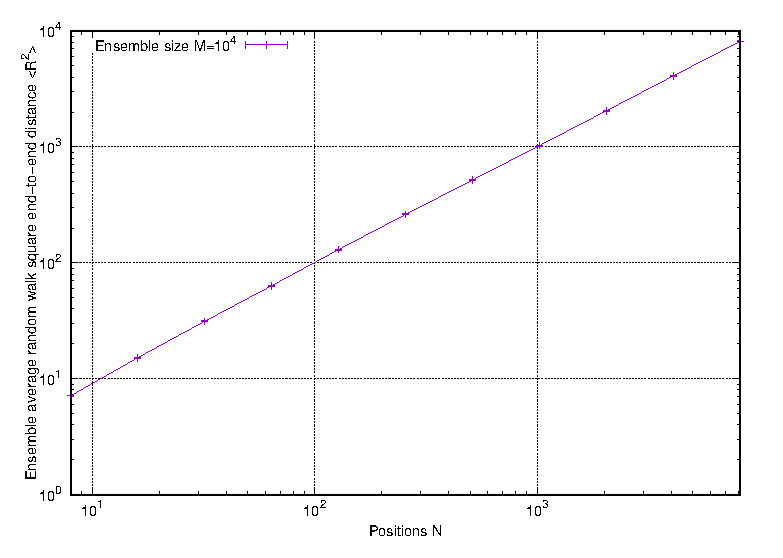
\includegraphics[scale=0.9]{figure1b.eps} 
\end{center}
\caption{Cube test for congruential random number generator with $c = 3, \: p = 31$.}
\label{fig:1b}
\end{figure}

\subsubsection{Subtask 1.3}
The random number generator was modified to run with $c = 2836, \: p = 127773$ to yield a substantially longer period and improved pseudo-randomness. As evident in figures~\ref{fig:1c}~and~\ref{fig:1d}, regular patterns appear much less common.


\begin{figure}[ht]
\begin{center}
\includegraphics[scale=0.9]{figure1c.eps} 
\end{center}
\caption{Square test for congruential random number generator with $c = 2836, \: p = 127773$.}
\label{fig:1c}
\end{figure}


\begin{figure}[ht]
\begin{center}
\includegraphics[scale=0.9]{figure1d.eps} 
\end{center}
\caption{Cube test for congruential random number generator with $c = 2836, \: p = 127773$.}
\label{fig:1d}
\end{figure}



\subsection{Task 2}
In polar coordinates, the angle $\phi$ can be chosen from a uniform distribution as the setup is invariant to rotation about the centre of the circle. The radius coordinate~$r$ however needs to be transformed $r \gets \sqrt{z} \;, \; z \sim \text{Unif} (0,1) $ as sampling from a uniform distribution would yield too much mass near the centre of the circle. Plotting 200 random numbers generated with $c = 2836, \: p = 127773$ on a circle with radius $R=1$ and center $(0, 0)$ yields the result shown in figure~\ref{fig:2}.

\begin{figure}[ht]
\begin{center}
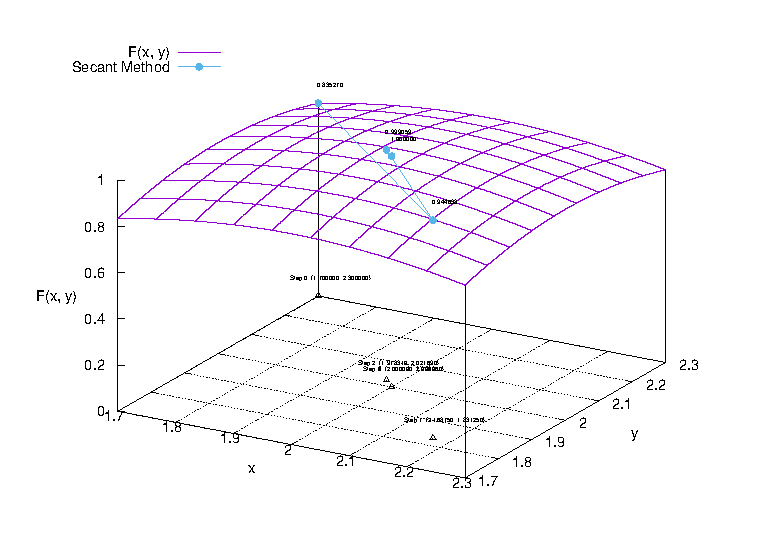
\includegraphics[scale=0.9]{figure2.eps} 
\end{center}
\caption{Output of congruential random number generator with $c = 2836, \: p = 127773$ plotted on circle with radius $R=1$ and center $(0, 0)$.}
\label{fig:2}
\end{figure}



\subsection{Task 3}
The code as submitted with this report was run several times to generate 2000 random numbers distributed over $k=10$ bins.\\
For $c = 3, \: p = 31$, the average score was $\chi^2 = 0.038$ which seems extremely unlikely when comparing to Knuth's table~\cite{knuth}.\\
For $c = 2836, \: p = 127773$, the average score was $\chi^2 = 6.778$ which is around the $p=40\%$ mark on Knuth's table~\cite{knuth}.\\
Clearly and as expected, $c = 3, \: p = 31$ make for a poor result in terms of randomness, whereas $c = 2836, \: p = 127773$ already achieve quite a respectable score. 

\section{Discussion}
The results were in line with the theoretical expectations from class. I personally had issues getting decent plots as I had shied away from Gnuplot until now. Also, my c++ is somewhat rusty and I apologise for my somewhat ugly code.

\begin{thebibliography}{99}


\bibitem{knuth}
  Knuth, Ervin D.,
  \emph{The art of computer programming}, 
  Addison Wesley, Massachusetts,
  3rd edition,
  1997.


\end{thebibliography}


\end{document}